\section{Producer-Consumer Model}

\subsection{The Need for Condition Variables}
\begin{frame}[fragile]{\emoji{sleeping} Why Not Just Use Busy-Waiting?}
	\textbf{Naive Approach: Polling}
	\begin{minted}{cpp}
std::queue<int> buffer;
std::mutex buffer_mutex;
bool done = false;

void consumer_busy_wait() {
    while (!done) {
        std::lock_guard<std::mutex> lock(buffer_mutex);
        if (!buffer.empty()) {
            int item = buffer.front();
            buffer.pop();
            std::cout << "Consumed: " << item << std::endl;
        }
        // Busy waiting - wastes CPU cycles!
    }
}
	\end{minted}

	\textbf{Problems}: CPU Waste • Power Drain • Lock Contention • Poor Scalability

	\emoji{bulb} \textbf{Solution}: Condition Variables - Sleep until notified!
\end{frame}

\subsection{Condition Variables}
\begin{frame}[fragile]{\emoji{bell} Condition Variables: Efficient Waiting}
	\textbf{Core Operations}:
	\begin{itemize}
		\item \texttt{wait(lock, predicate)}: Sleep until condition is true
		\item \texttt{notify\_one()}: Wake up one waiting thread
		\item \texttt{notify\_all()}: Wake up all waiting threads
	\end{itemize}

	\vspace{0.5em}
	\textbf{Basic Pattern}:
	\begin{minted}{cpp}
std::mutex mtx;
std::condition_variable cv;
bool ready = false;

void waiter() {
    std::unique_lock<std::mutex> lock(mtx);
    cv.wait(lock, []{ return ready; });  // Sleep until ready
    std::cout << "Condition met!" << std::endl;
}

void notifier() {
    {
        std::lock_guard<std::mutex> lock(mtx);
        ready = true;  // Set condition
    }
    cv.notify_one();  // Wake up waiter
}
	\end{minted}

	\textbf{Key Points}: Use \texttt{unique\_lock} • Always use predicate • Modify before notify
\end{frame}

\begin{frame}[fragile]{\emoji{gear} How Condition Variables Work}
	\textbf{Internal Mechanism}:

	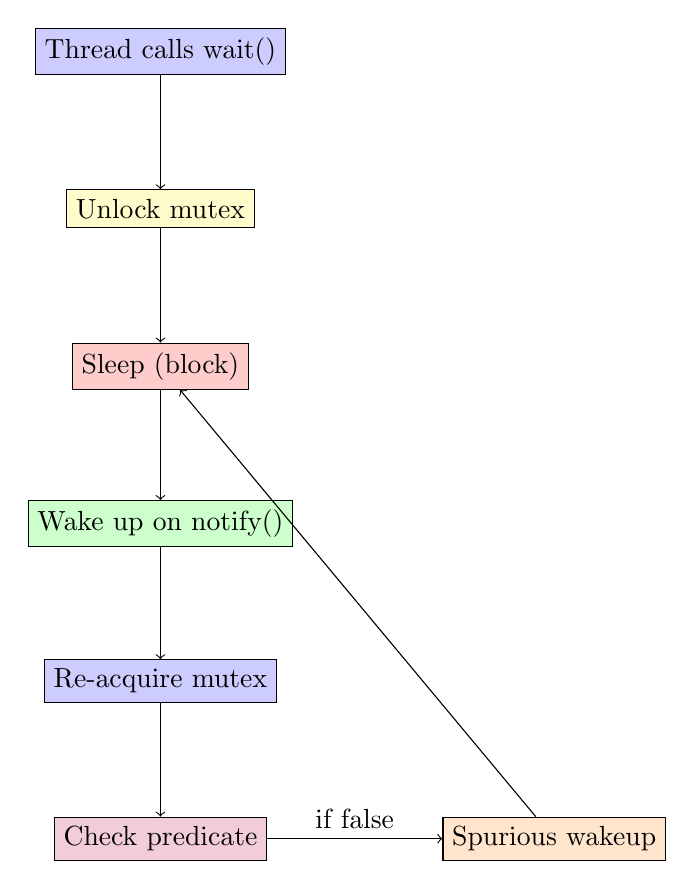
\begin{tikzpicture}[node distance=2cm]
		% Nodes
		\node[draw, rectangle, fill=blue!20] (thread) {Thread calls wait()};
		\node[draw, rectangle, fill=yellow!20, below of=thread] (unlock) {Unlock mutex};
		\node[draw, rectangle, fill=red!20, below of=unlock] (sleep) {Sleep (block)};
		\node[draw, rectangle, fill=green!20, below of=sleep] (wakeup) {Wake up on notify()};
		\node[draw, rectangle, fill=blue!20, below of=wakeup] (relock) {Re-acquire mutex};
		\node[draw, rectangle, fill=purple!20, below of=relock] (check) {Check predicate};
		\node[draw, rectangle, fill=orange!20, right of=check, xshift=3cm] (spurious) {Spurious wakeup};

		% Arrows
		\draw[->] (thread) -- (unlock);
		\draw[->] (unlock) -- (sleep);
		\draw[->] (sleep) -- (wakeup);
		\draw[->] (wakeup) -- (relock);
		\draw[->] (relock) -- (check);
		\draw[->] (check) -- node[above] {if false} (spurious);
		\draw[->] (spurious) -- (sleep);
	\end{tikzpicture}

	\vspace{0.5em}
	\textbf{Why Use Predicates?}
	\begin{minted}{cpp}
// Vulnerable to spurious wakeups
cv.wait(lock);
if (condition) { /* work */ }

// Robust against spurious wakeups
cv.wait(lock, []{ return condition; });
// Equivalent to:
while (!condition) {
    cv.wait(lock);
}
	\end{minted}
\end{frame}

\subsection{Thread-Safe Queue Implementation}
\begin{frame}[fragile]{\emoji{package} Thread-Safe Queue: Structure}
	\textbf{Class Definition}:

	\begin{minted}{cpp}
template<typename T>
class ThreadSafeQueue {
private:
    std::queue<T> queue_;
    mutable std::mutex mutex_;
    std::condition_variable condition_;

public:
    void push(const T& item);
    T pop();  // Blocks until item available
    bool empty() const;
    size_t size() const;
};
	\end{minted}
\end{frame}

\begin{frame}[fragile]{\emoji{package} Thread-Safe Queue: Implementation}
	\textbf{Core Methods}:

	\begin{minted}{cpp}
void push(const T& item) {
    {
        std::lock_guard<std::mutex> lock(mutex_);
        queue_.push(item);
    }
    condition_.notify_one();  // Wake up waiting consumers
}

T pop() {
    std::unique_lock<std::mutex> lock(mutex_);
    condition_.wait(lock, [this] { return !queue_.empty(); });

    T item = queue_.front();
    queue_.pop();
    return item;
}
	\end{minted}
\end{frame}

\subsection{Producer-Consumer Implementation}
\begin{frame}[fragile]{\emoji{factory} Producer-Consumer: Simplified Example}
	\begin{minted}{cpp}
ThreadSafeQueue<int> shared_queue;
bool done = false;

void producer(int id, int num_items) {
    for (int i = 0; i < num_items; ++i) {
        int item = rand() % 100;
        shared_queue.push(item);
        std::cout << "Producer " << id << " produced: " << item << std::endl;

        std::this_thread::sleep_for(std::chrono::milliseconds(100));
    }
}

void consumer(int id) {
    while (!done) {
        int item = shared_queue.pop();  // Blocks until available
        std::cout << "Consumer " << id << " consumed: " << item << std::endl;

        std::this_thread::sleep_for(std::chrono::milliseconds(150));
    }
}
	\end{minted}
\end{frame}

\begin{frame}[fragile]{\emoji{rocket} Running the System}
	\begin{minted}{cpp}
int main() {
    std::vector<std::thread> threads;

    // Start 3 consumers
    for (int i = 0; i < 3; ++i) {
        threads.emplace_back(consumer, i);
    }

    // Start 2 producers
    for (int i = 0; i < 2; ++i) {
        threads.emplace_back(producer, i, 5);  // 5 items each
    }

    // Wait for producers to finish (simplified)
    std::this_thread::sleep_for(std::chrono::seconds(3));
    done = true;  // Signal consumers to stop

    // Wait for all threads
    for (auto& t : threads) {
        t.join();
    }

    return 0;
}
	\end{minted}

	\textbf{Benefits}: Efficient waiting • No busy loops • Thread-safe communication
\end{frame}

\begin{frame}[fragile]{\emoji{chart-increasing} Performance Comparison}
	\textbf{Busy-Waiting vs Condition Variables}

	\begin{table}[h]
		\centering
		\begin{tabular}{|l|c|c|}
			\hline
			\textbf{Metric}   & \textbf{Busy-Waiting} & \textbf{Condition Variables} \\
			\hline
			CPU Usage         & 95-100\%              & 5-15\%                       \\
			Response Time     & Low                   & Low                          \\
			Throughput        & Medium                & High                         \\
			Power Consumption & High                  & Low                          \\
			Scalability       & Poor                  & Good                         \\
			\hline
		\end{tabular}
	\end{table}

	\vspace{1em}
	\textbf{Real-world Applications}:
	\begin{itemize}
		\item \textbf{Web Servers}: Request queue processing
		\item \textbf{Database Systems}: Transaction queue management
		\item \textbf{Game Engines}: Event processing pipelines
		\item \textbf{Media Players}: Audio/video buffer management
	\end{itemize}
\end{frame}
